% Tableaux de résultats, graphiques
% Préciser l'erreur
% Incertitudes

Ayant toutes les vidéos prises pour les différentes masses et rayons, il a fallu effectuer le tracking du point qui tourne. Pour cela nous avons utilisé la librairie \emph{Python} nommée \textit{OpenCV}\footnote{\href{opencv.org}{Site internet : \textit{opencv.org}}}.\\ 
\begin{invsummary}
\textit{OpenCV} est la plus grande librairie d'analyse vidéo. C'est open source et contient plus de 2500 algorithmes. Elle est écrite en \emph{C} et est supportée également en \emph{C++}, \emph{Java} et \emph{Python}. On peut également noté un support de toute les plateformes principales (\textit{Windows}, \textit{Linux}, \textit{MacOS}), les mobiles (\textit{Android}, \textit{iOS}) mais surtout les interfaces graphiques majeurs (\textit{CUDA}, \textit{OpenCL}).
\end{invsummary}
Nous avons donc importé les vidéos avec cette librairie afin de les convertir en liste de matrices de pixels pour chaque image, qui peuvent être visualisée par \textit{matplotlib} et manipulée comme des \textit{array} de \textit{numpy}. Nous avons pris aussi le nombre d'images par seconde ($[fps]$). Pour les trois mesures à $70 \ [g]$, nous avons essayé de l'augmenté en prenant des vidéos via le ralenti d'un \textit{iPhone}, qui est selon le constructeur du $120 \ [fps]$, mais sont encodée ensuite en $30 \ [fps]$, et pas de manière régulière (vidéo qui ralenti au fur et à mesure puis accélère à la fin dans un but esthétique) ce qui explique le grand étalement des vitesse. Toutes les autres mesures sont en $60 \ [fps]$ standards.\\
Nous avons ensuite sélectionné la partie de la vidéo que l'on désire analyser, et sur la première image de celle-ci nous avons repérer dans un carré de 50 pixels la position du centre et du point de tracking sur le disque. Nous avons ensuite enregistrer les positions sur chaque image du point via un algorithme \textit{CSRT}\footnote{\href{https://medium.com/@khwabkalra1/object-tracking-2fe4127e58bf}{Fonctionnement de CSRT : \textit{https://medium.com/@khwabkalra1/object-tracking-2fe4127e58bf}}}. Comme la position est enregistrée comme un rectangle de coins supérieur gauche $(a,b)$ et de dimension $w \times h$, on peut le transformer en un point $(x,y) = (\frac{x+(x+w)}{2},\frac{y+(y+h)}{2})$.\\
\begin{summary}
L'algorithme \textit{CSRT} (\textit{Channel and Spatial Reliability Tracker}) est un algorithme de tracking assez lent, mais très précis et robuste. Il s'appuie sur la couleur pour une meilleur stabilité, ainsi que sur l'évolution spatiale et temporel de l'objet. Il utilise un filtre de corrélation pour estimer la position de l'objet, et ce filtre est entraîné et mis à jour itérativement durant le tracking.
\end{summary}
Connaissant donc la position du centre de rotation $(x_c,y_c)$ ainsi que la position du point de tracking à chaque image $(x_f, y_f)$, ainsi que le temps entre deux images $\Delta t$ qui est l'inverse du nombre d'image par seconde, nous pouvons calculer la position angulaire du point de tracking par rapport au centre et sa position initiale au court du temps. Pour cela, nous utilisons la formule $\theta_{f+1} = \theta_f + \arctan(\frac{y_f}{x_f}) - \arctan(\frac{y_{f-1}}{x_{f-1}})$ avec $\theta_f$ la position angulaire à chaque frame et l'$\arctan$ est celle prenant en compte le cadrant. Afin de corriger les saut de $2\pi$ après un tour complet, nous avons corrigé les valeurs quand $|\arctan(\frac{y_f}{x_f}) - \arctan(\frac{y_{f-1}}{x_{f-1}})|$ est supérieur à $\pi$ (comme nos angles sont assez petit c'est une borne suffisante) par $\theta_f := \theta_f - 2\pi \cdot sgn(\arctan(\frac{y_f}{x_f}) - \arctan(\frac{y_{f-1}}{x_{f-1}}))$, avec $sgn(x) = \begin{cases} 1 & \text{si } x \geq 0 \\ -1 & \text{si } x < 0 \end{cases}$. Nous avons alors à ce stade les couples angles-temps $((\theta_0, 0),(\theta_1, \Delta t),...,(\theta_f, f \cdot \Delta t),...)$ qui forment notre fonction. Nous avons donc fait une courbe de tendance quadratique ($ax^2 + bx + c$) ensuite par la méthode des moindres carrés. Finalement, par la théorie du mouvement circulaire uniformément accéléré (\textit{MCUA}), nous pouvons calculer l'accélération angulaire $\alpha$ en doublant le coefficient pour $x^2$ dans notre courbe de tendance.\\ \\
Pour la vitesse angulaire, nous avons fait une dérivée numérique : $\omega_f = \frac{\theta{f+1} - \theta_f}{\Delta t}$, puis fait une courbe de tendance linéaire ($ax+b$) avec les couples vitesse-temps obtenus. Le coefficient pour $x$ est par le \textit{MCUA} l'accélération angulaire. Nous avons refait cela afin d'obtenir accélération angulaire instantanée, mais les résultats sont trop aléatoires pour être exploités. Les figures suivantes présentent les trois graphes ($\theta(t)$, $\omega(t)$ et $\alpha{t}$, selon le temps $t$) pour chaque mesure en précisant la masse et le rayon considéré (celui dit petit est de $1.5 \ [cm]$, moyen $3 \ [cm]$ et grand $4.5 \ [cm]$). Les mesures sont en bleu et les courbes de tendances en vert. Leurs paramètres sont disponibles dans le \textit{notebook} de calculs fourni en annexe.

\begin{figure}[H]
\centering
\begin{subfigure}[t]{.3\linewidth}
\centering
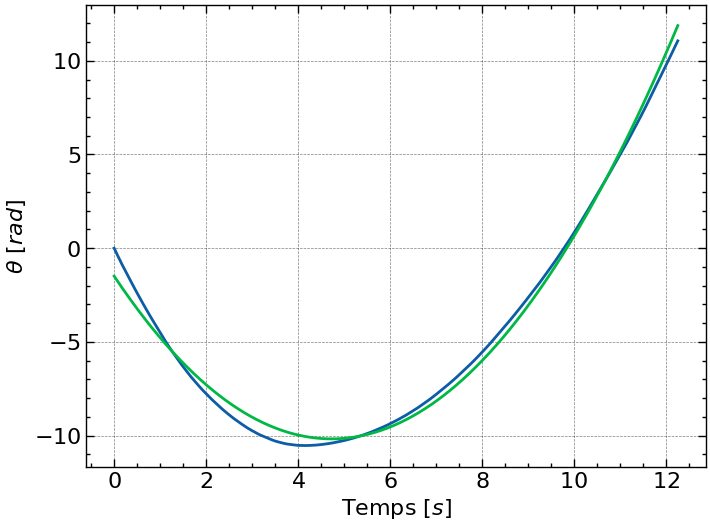
\includegraphics[width=.9\linewidth]{m40_t}
\end{subfigure}
\begin{subfigure}[t]{.3\linewidth}
\centering
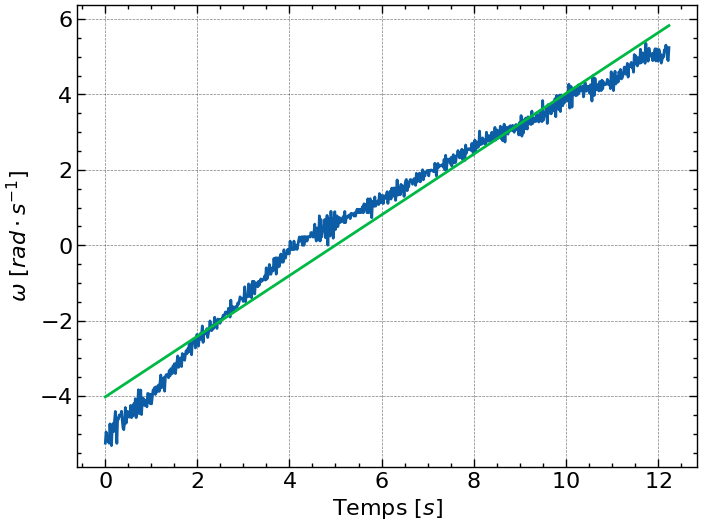
\includegraphics[width=.9\linewidth]{m40_o}
\end{subfigure}
\begin{subfigure}[t]{.3\linewidth}
\centering
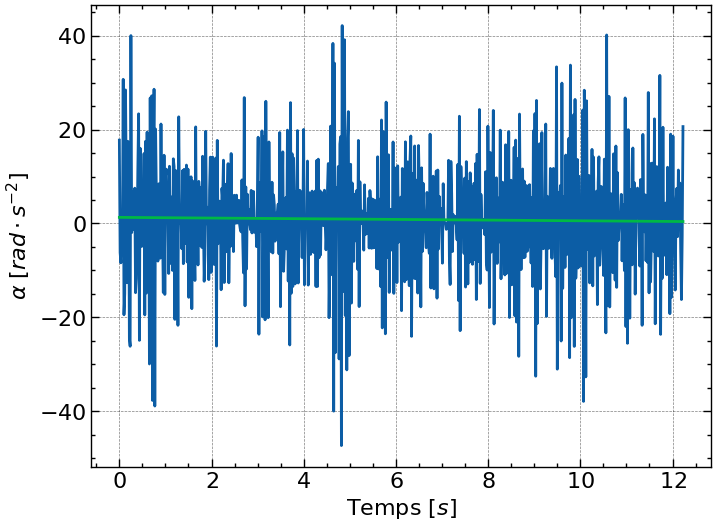
\includegraphics[width=.9\linewidth]{m40_a}
\end{subfigure}
\caption{Angle, vitesse angulaire et accélération angulaire pour une masse de $40 \ [g]$ sur le rayon moyen}
\label{fig:m40}
\end{figure}

\begin{figure}[H]
\centering
\begin{subfigure}[t]{.3\linewidth}
\centering
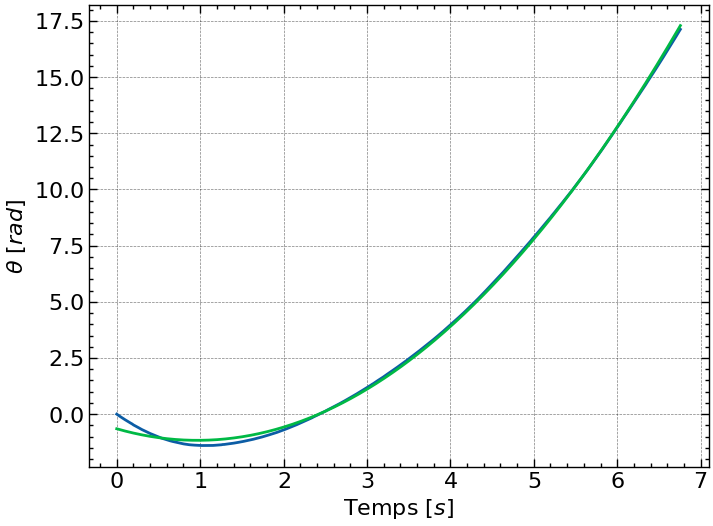
\includegraphics[width=.9\linewidth]{m60_t}
\end{subfigure}
\begin{subfigure}[t]{.3\linewidth}
\centering
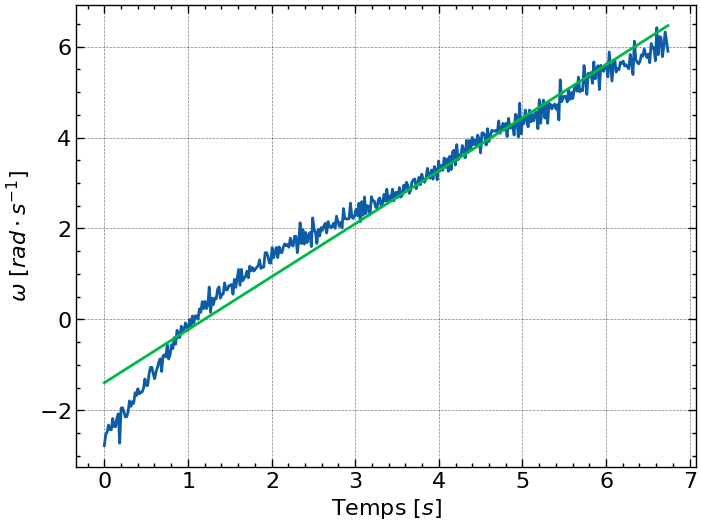
\includegraphics[width=.9\linewidth]{m60_o}
\end{subfigure}
\begin{subfigure}[t]{.3\linewidth}
\centering
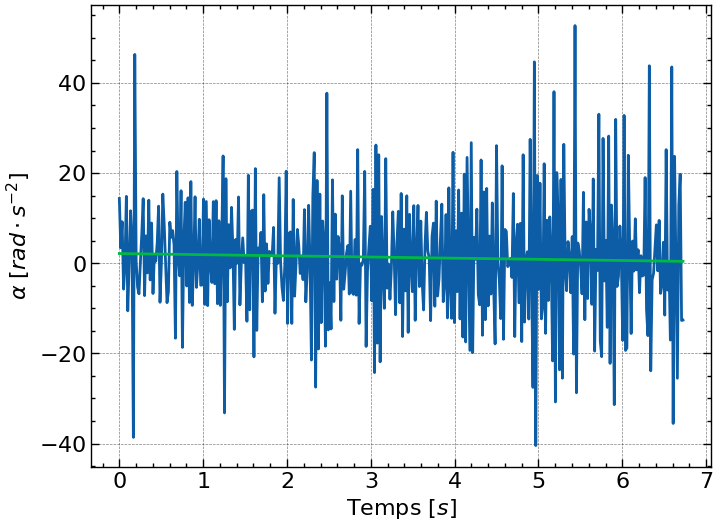
\includegraphics[width=.9\linewidth]{m60_a}
\end{subfigure}
\caption{Angle, vitesse angulaire et accélération angulaire pour une masse de $60 \ [g]$ sur le rayon moyen}
\label{fig:m60}
\end{figure}

\begin{figure}[H]
\centering
\begin{subfigure}[t]{.3\linewidth}
\centering
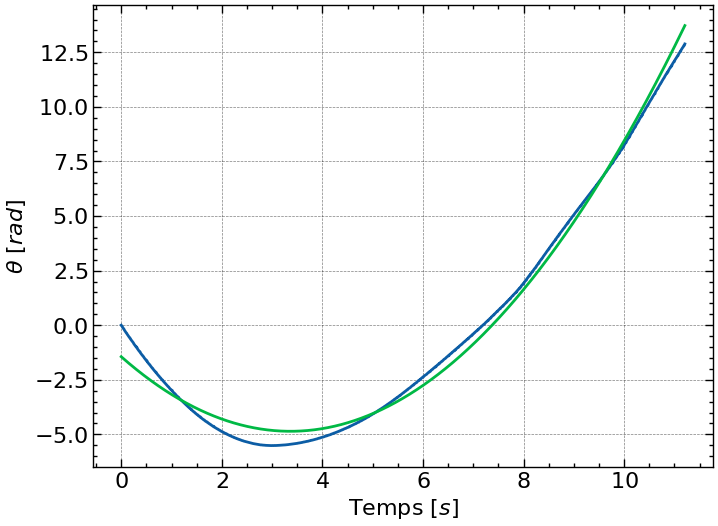
\includegraphics[width=.9\linewidth]{p70_t}
\end{subfigure}
\begin{subfigure}[t]{.3\linewidth}
\centering
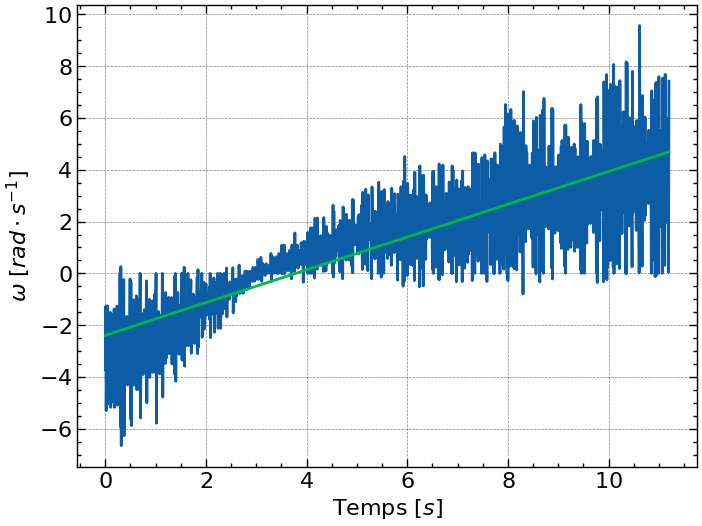
\includegraphics[width=.9\linewidth]{p70_o}
\end{subfigure}
\begin{subfigure}[t]{.3\linewidth}
\centering
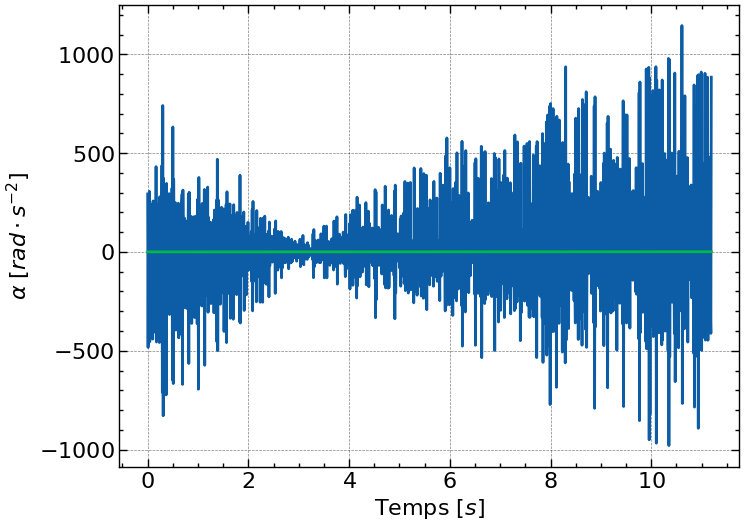
\includegraphics[width=.9\linewidth]{p70_a}
\end{subfigure}
\caption{Angle, vitesse angulaire et accélération angulaire pour une masse de $70 \ [g]$ sur le rayon petit}
\label{fig:p70}
\end{figure}

\begin{figure}[H]
\centering
\begin{subfigure}[t]{.3\linewidth}
\centering
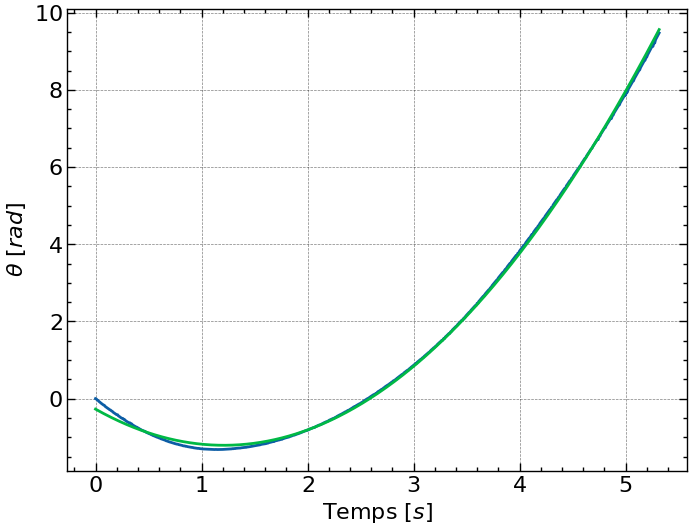
\includegraphics[width=.9\linewidth]{m70_t}
\end{subfigure}
\begin{subfigure}[t]{.3\linewidth}
\centering
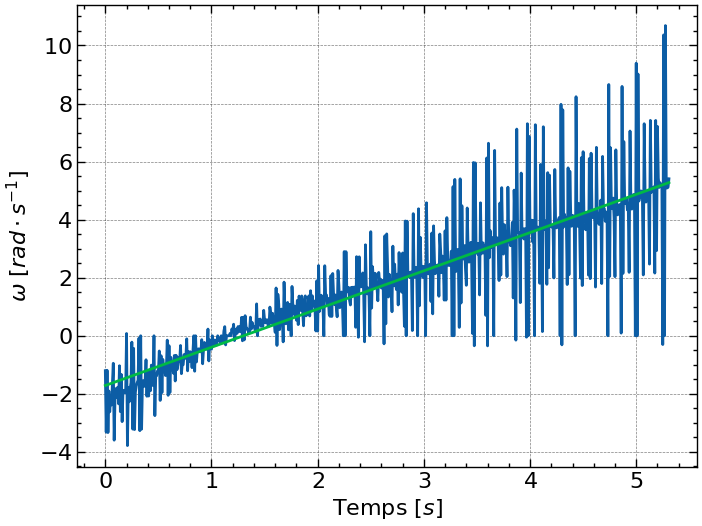
\includegraphics[width=.9\linewidth]{m70_o}
\end{subfigure}
\begin{subfigure}[t]{.3\linewidth}
\centering
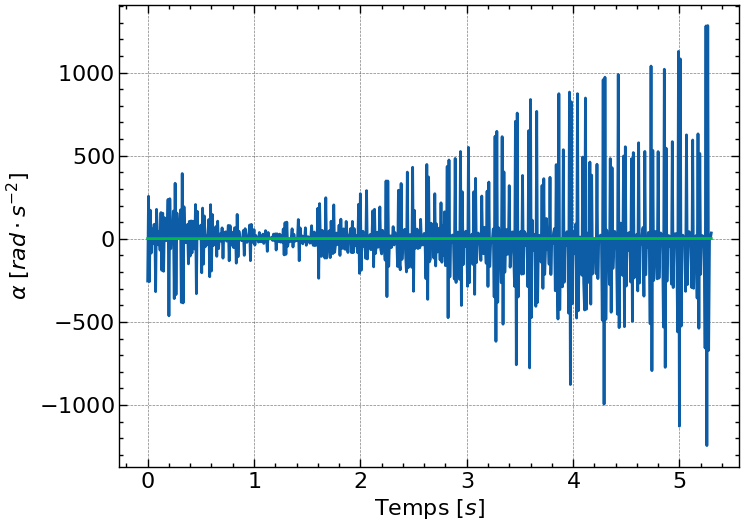
\includegraphics[width=.9\linewidth]{m70_a}
\end{subfigure}
\caption{Angle, vitesse angulaire et accélération angulaire pour une masse de $70 \ [g]$ sur le rayon moyen}
\label{fig:m70}
\end{figure}

\begin{figure}[H]
\centering
\begin{subfigure}[t]{.3\linewidth}
\centering
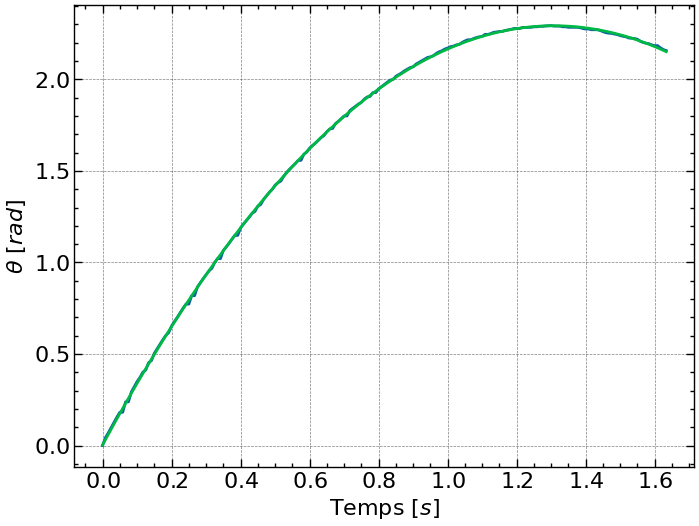
\includegraphics[width=.9\linewidth]{g70_t}
\end{subfigure}
\begin{subfigure}[t]{.3\linewidth}
\centering
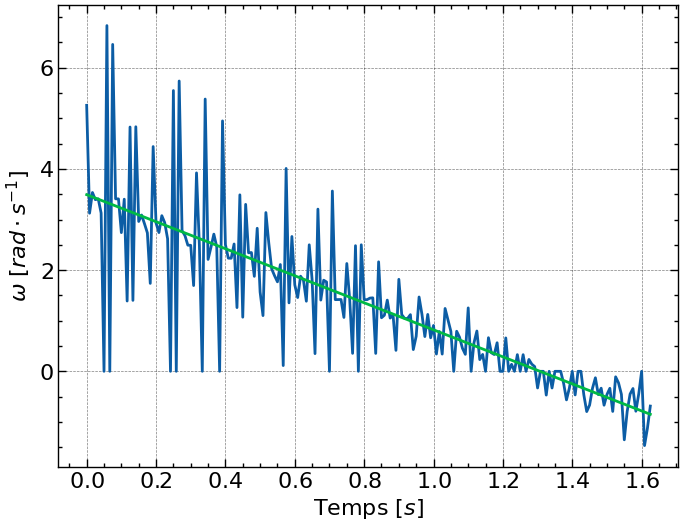
\includegraphics[width=.9\linewidth]{g70_o}
\end{subfigure}
\begin{subfigure}[t]{.3\linewidth}
\centering
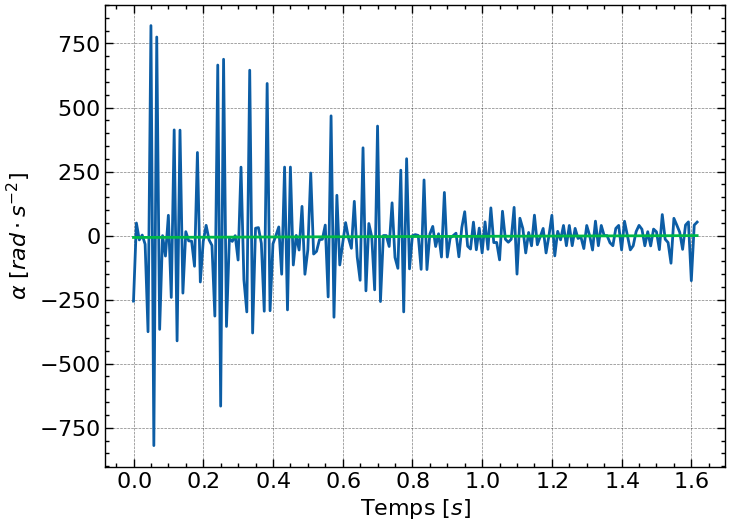
\includegraphics[width=.9\linewidth]{g70_a}
\end{subfigure}
\caption{Angle, vitesse angulaire et accélération angulaire pour une masse de $70 \ [g]$ sur le rayon grand}
\label{fig:g70}
\end{figure}

\begin{figure}[H]
\centering
\begin{subfigure}[t]{.3\linewidth}
\centering
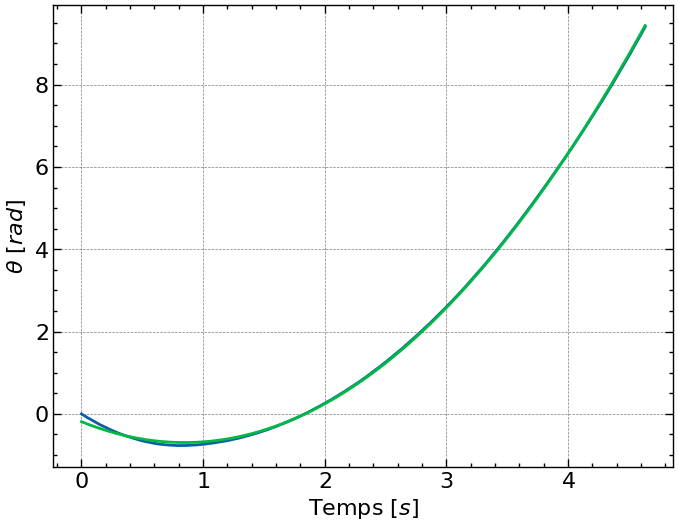
\includegraphics[width=.9\linewidth]{m80_t}
\end{subfigure}
\begin{subfigure}[t]{.3\linewidth}
\centering
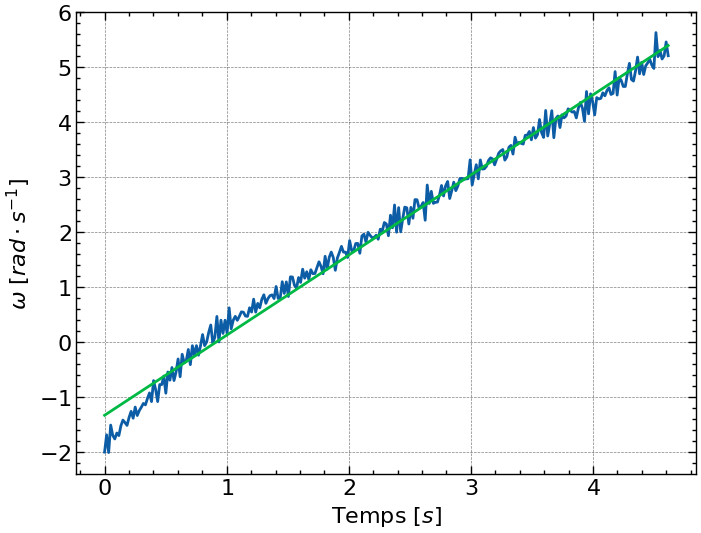
\includegraphics[width=.9\linewidth]{m80_o}
\end{subfigure}
\begin{subfigure}[t]{.3\linewidth}
\centering
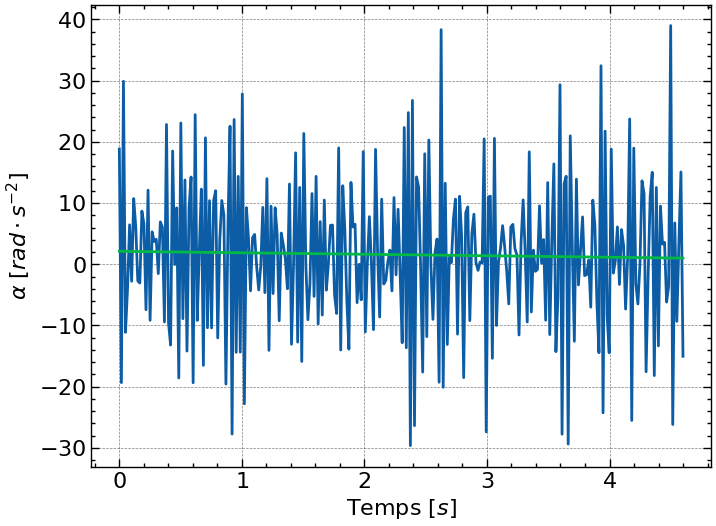
\includegraphics[width=.9\linewidth]{m80_a}
\end{subfigure}
\caption{Angle, vitesse angulaire et accélération angulaire pour une masse de $80 \ [g]$ sur le rayon moyen}
\label{fig:m80}
\end{figure}

\begin{figure}[H]
\centering
\begin{subfigure}[t]{.3\linewidth}
\centering
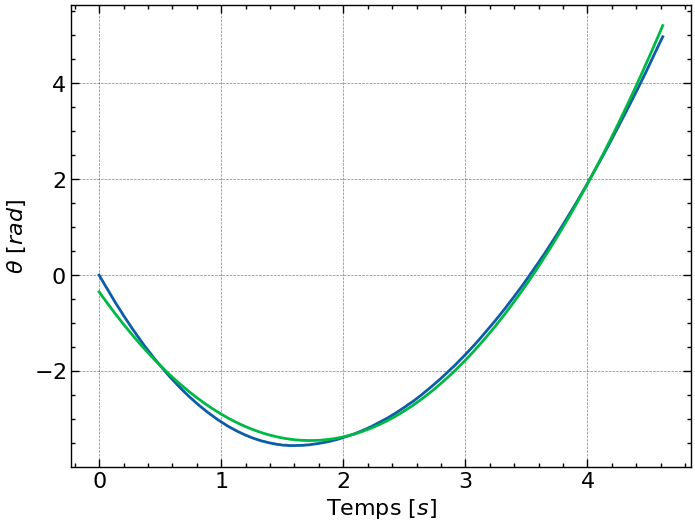
\includegraphics[width=.9\linewidth]{m100_t}
\end{subfigure}
\begin{subfigure}[t]{.3\linewidth}
\centering
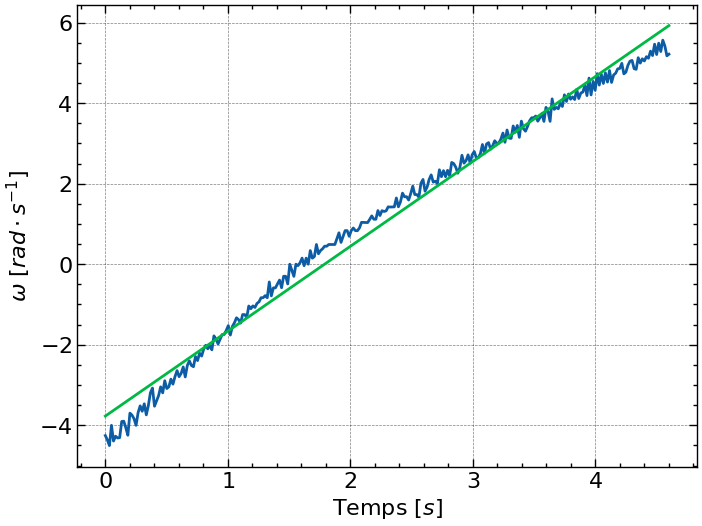
\includegraphics[width=.9\linewidth]{m100_o}
\end{subfigure}
\begin{subfigure}[t]{.3\linewidth}
\centering
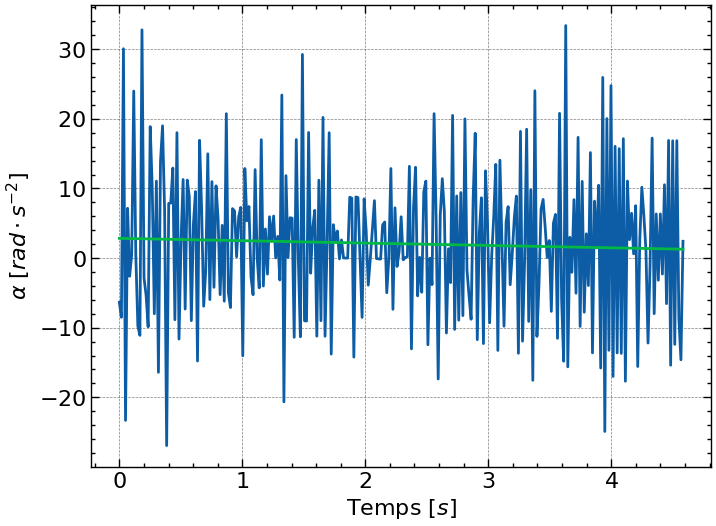
\includegraphics[width=.9\linewidth]{m100_a}
\end{subfigure}
\caption{Angle, vitesse angulaire et accélération angulaire pour une masse de $100 \ [g]$ sur le rayon moyen}
\label{fig:m100}
\end{figure}

Nous avons finalement consignés les principaux résultats dans la table suivante. Nous avons utilisé comme accélération angulaire la moyenne de celle obtenue par $\theta$ et celle par $\omega$ sans consigné outre mesure les valeurs particulières comme elles sont très proches (autour de 1 à 5 $[\%]$ d'écart, avec une autour de 10 $[\%]$), mais elles sont également visibles dans le \textit{notebook}. Le moment d’inertie du disque à été calculé dans chaque cas en considérant que la seul force $F$ créant un moment est celle de pesanteur du contrepoids de masse $m$ parfaitement redirigée par une poulie sans frottement et s'appliquant perpendiculairement au rayon. Pour le rayon $r$, on aura donc le moment $M = F \cdot r = mgr$ avec $g = 9.81 \ [m \cdot s^{-2}]$ d'où la relation $M=I\alpha \Leftrightarrow I = \frac{M}{\alpha}$.

\begin{table}[H]
\centering
\begin{tabular}{rrrr}
\toprule
 $m \ [kg]$ &  $r \ [m]$ &  $I \ [kg \cdot m^2]$ &  $\alpha \ [rad \cdot s^{-2}]$ \\
\midrule
  0.040 &  0.030 &      0.015 &            0.791 \\
  0.060 &  0.030 &      0.016 &            1.133 \\
  0.070 &  0.015 &      0.017 &            0.618 \\
  0.070 &  0.030 &      0.016 &            1.297 \\
  0.070 &  0.045 &      0.012 &            2.673 \\
  0.080 &  0.030 &      0.016 &            1.435 \\
  0.100 &  0.030 &      0.014 &            2.092 \\
\bottomrule
\end{tabular}
\caption{Récapitulatif des principaux résultats}
\label{tab:recap}
\end{table}

Comme le disque est toujours le même avec le même axe de rotation, le moment d'inertie est censé être constant, ce qui se voit par une moyenne de $I \approx 0.015 \ [kg \cdot m^2]$ avec un écart-type de $0.0016$ qui correspond à moins de $11 \ [\%]$. Par les relations précédentes, nous voyons que $\alpha$ dépend linéairement de la masse et du rayon car le moment de force l'est que $I$ est constant, ce qui est illustré par la figure suivante.

\begin{figure}[H]
\centering
\begin{subfigure}[t]{.45\linewidth}
\centering
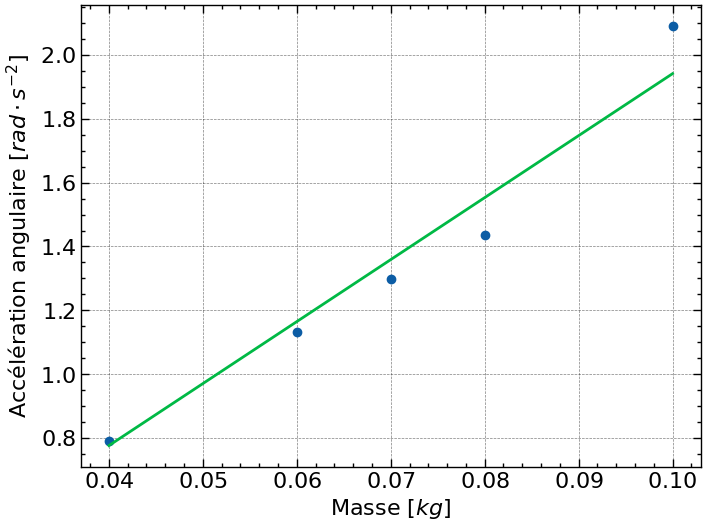
\includegraphics[width=.9\linewidth]{prop_masse}
\caption{Rayon moyen}
\end{subfigure}
\begin{subfigure}[t]{.45\linewidth}
\centering
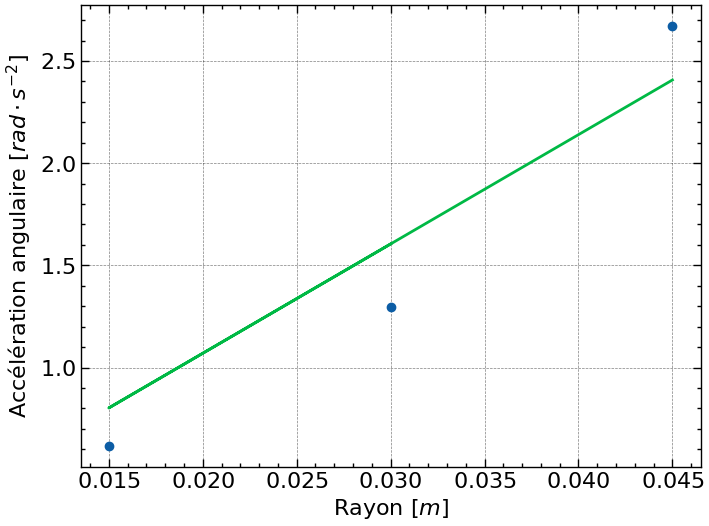
\includegraphics[width=.9\linewidth]{prop_rayon}
\caption{Masse de $70 \ [g]$}
\end{subfigure}
\caption{Accélération angulaire selon un paramètre fixé}
\label{fig:prop}
\end{figure}
